\chapter{Data and Research Context}
\label{chap:data-and-research-context}

\section{Research Context: WeiMai Social Marketing System}
\label{sec:3-1-research-context-weimai-social-marketing-system}

The data analysed in this dissertation are generated through the WeiMai social marketing system. WeiMai operates a marketing system that serves business customers with marketing needs. The empirical records used in this study come from Mingjiang ({\cjkfont 名匠}), a single interior-design company that used the system for WeChat-based marketing activity in 2016–2017. In this dissertation, WeiMai is treated as the data environment through which Mingjiang’s article-sharing, reading, and resharing behaviours were recorded.

A key advantage of the WeiMai records is that they contain behavioural traces of the sharing process. The dataset includes reading events, reading duration, reshare behaviour, and linkage information identifying the prior share through which a reader was reached. These linkage fields make it possible to reconstruct each article–agent sharing case into a diffusion cascade. This distinguishes the WeiMai records used in this dissertation from platform-level aggregate statistics, which may report total views or total shares but do not show how an article moved through a network after being distributed.

Mingjiang’s marketing content is related to interior design, home decoration, and real-estate-related services. This setting is suitable for examining content–agent fit since marketing communication in this industry is closely connected to professional relevance, visual presentation, trust, and topic familiarity. Articles may discuss home design and decoration, real estate and architecture, events and promotions, brand and marketing, lifestyle and culture, or customer service and management. These topics are unlikely to be equally relevant to all agents or to all audience contexts.

In this empirical setting, marketing agents serve as the observed entry points through which article diffusion begins. Each agent-linked article-sharing case exposes an article to a surrounding WeChat audience, and any subsequent resharing may carry the article further into the network. The agent has a dual role in the data. On the one hand, the agent is an organisational representative participating in Mingjiang’s marketing activity. On the other hand, the agent is the origin point of an observed diffusion process, because later reading and sharing records can be linked to the agent-mediated dissemination path.

This context is directly connected to the dissertation’s concern with personalised content assignment. A uniform distribution strategy treats agents as interchangeable channels and distributes the same content broadly, regardless of topic relevance or agent context. The WeiMai records allow this assumption to be examined empirically because they contain variation across articles, across agents, and across agent–topic combinations. Some articles may perform better on average, some agents may show stronger average diffusion outcomes, and some content topics may be more effective when shared by agents whose professional contexts are better aligned with those topics.

Throughout this dissertation, the WeiMai records are treated as observational records of a live marketing operation, not as the product of a controlled experiment. The data make it possible to examine systematic associations between content, agents, content–agent fit, and diffusion effectiveness, but they do not by themselves identify causal effects. The data sources, cleaning scope, units of analysis, outcome variables, and limitations together support the three-level empirical framework.

\section{Raw Data Sources}
\label{sec:3-2-raw-data-sources}

The empirical analysis is based on three main groups of raw data sources connected to the focal interior-design company’s WeChat marketing activity, including WeChat reading and sharing records, article content files, and agent organisational profile and identifier records.

The first raw data source is the WeChat reading and sharing log recorded through the WeiMai system. This log was read from the database table \emph{detail} and exported locally as \emph{detail.csv} during Stage 1. Each record is associated with an article and an agent, and records the reader involved, the time of the reading event, the time spent on the article, the reading status, and whether the reader reshared the article. The key fields include \varname{article\_title},\allowbreak{} \varname{agent\_name},\allowbreak{} \varname{reader\_wechat\_nn},\allowbreak{} \varname{reader\_layer},\allowbreak{} \varname{reader\_address},\allowbreak{} \varname{reader\_gender},\allowbreak{} \varname{reader\_time},\allowbreak{} \varname{reader\_stay},\allowbreak{} \varname{reader\_share2moment},\allowbreak{} \varname{reader\_share2friend},\allowbreak{} \varname{reader\_read},\allowbreak{} and \varname{network\_parent}.

This behavioural log is central to the dissertation because it allows diffusion to be studied as a process, not as a single exposure count. The \varname{reader\_stay} field records dwell time, while \varname{reader\_share2moment} and \varname{reader\_share2friend} indicate whether a reader reshared the article to WeChat Moments or to friends. The \varname{reader\_layer} and \varname{network\_parent} fields provide the linkage information needed to identify how a reader was reached in the observed propagation sequence. These fields later support cascade reconstruction and layer correction.

The second raw data source is the article content corpus. The marketing articles are stored in a local folder as individual Word/DOCX files. Each file contains the article title, body text, and, where present, embedded images. These files provide the original content material for the study. They are later processed to construct content-side variables such as article topic, title–content semantic consistency, word count, image presence, and image count through the Stage 2 content-processing workflow.

The third raw data source is the agent organisational profile and WeChat identifier data. These records were read from the database tables \emph{agent\_dep\_job} and \emph{agent\_wechatnn} and exported locally as \emph{agent\_dep\_job.csv} and \emph{agent\_wechatnn.csv}. The organisational profile records contain agent names, department information, and job titles. These fields provide the basis for describing agents’ observable professional contexts. In addition, agent WeChat identifier records are used to link organisational agents with the WeChat behavioural records through their nicknames. This study connects article-sharing and reading behaviour to the agents through whom the articles entered the WeChat environment.

Together, these three raw sources define the empirical foundation of the dissertation. The WeChat behavioural log records how articles were read and reshared; the DOCX article corpus records what the articles contained; and the agent profile and identifier records connect observed sharing behaviour to organisational agents and their professional roles. Later outputs, including cleaned behavioural datasets, LLM-generated content features, corrected diffusion cascades, and three-level analysis-ready datasets, are derived from these raw sources and are not treated as raw inputs.

\begin{table}[H]
\centering
\scriptsize
\caption{Raw Data Sources Used in the Study}
\label{tab:3-1}
\renewcommand{\arraystretch}{1.15}
\begin{tabularx}{\textwidth}{>{\raggedright\arraybackslash}p{0.21\textwidth}>{\raggedright\arraybackslash}p{0.22\textwidth}>{\raggedright\arraybackslash}p{0.28\textwidth}>{\raggedright\arraybackslash}p{0.20\textwidth}}
\toprule
\textbf{Raw data source} & \textbf{Main file/table} & \textbf{Key contents} & \textbf{Role in the study} \\
\midrule
WeChat reading and sharing log & Database table \emph{detail}; local export \emph{detail.csv} & Article, agent, reader, layer, gender, time, dwell-time, read, reshare, and parent-link fields & Reading, resharing, and propagation paths \\
Article DOCX content files & Local folder of article Word/DOCX files & Article titles, body text, and embedded images & Article content feature construction \\
Agent profile and WeChat identifier records & \makecell[l]{Database tables\\ \emph{agent\_dep\_job}\\ \emph{agent\_wechatnn}\\ Local exports\\ \emph{agent\_dep\_job.csv}\\ \emph{agent\_wechatnn.csv}} & Names, departments, job titles, and WeChat nicknames & Agent context and ID linkage \\
\bottomrule
\end{tabularx}
\end{table}

\section{Raw Data Scale and Cleaning Scope}
\label{sec:3-3-raw-data-scale-and-cleaning-scope}

The raw data sources differ in scale and structure. The largest source is the WeChat reading and sharing log generated through the WeiMai system, which provides the original records for observing article reading, dwell time, resharing, and propagation linkage. The exact size of this raw export was not separately recorded. The first quantified count is the table retained after the initial agent-linkage filtering, described below. The article content source consists of 1,423 original Word/DOCX documents, while the agent source consists of organisational profile records and WeChat identifier records used to connect agents to the behavioural log. Because these sources are observed at different levels, they must be cleaned, linked, and reorganised before empirical analysis.

The first part of the cleaning process restricts the behavioural records to observations that can be linked to valid agent information. The original behavioural source is the database table \emph{detail}, with a local exported version stored as \emph{detail.csv}. After the initial reader and agent linkage filtering, the retained behavioural table, labelled \varname{detail\_filtered1} in the processing notes, contains 258,179 rows. This step removes records that cannot be connected consistently to the agent profile and identifier information needed for later agent-level and content–agent analyses.

The second part of the cleaning process restricts the behavioural records to articles with available content files. Since the dissertation studies the relationship between article content and diffusion outcomes, a behavioural record can only be used in the content-linked analysis if its article can be connected to a corresponding DOCX file. After this linkage restriction, the main content-linked behavioural table, \emph{detail\_filtered2.xlsx}, contains 209,895 rows and 13 columns. These records form the main event-level behavioural foundation carried forward into diffusion reconstruction.

The third part of the cleaning process concerns propagation-layer correction. The raw behavioural log includes reader-layer and parent-linkage fields, but these fields require correction before cascade-level measures can be computed reliably. After layer correction and cascade reconstruction, the corrected reader-level diffusion file, \emph{diffusion\_corrected\_layers.xlsx}, contains 199,154 rows and 23 columns. This file provides the corrected propagation-layer records used to construct later diffusion outcomes.

The article content scope also changes across stages. The raw article corpus contains 1,423 original Word/DOCX documents. After title/path indexing, the article inventory contains 1,421 unique article titles, indicating that the number of raw files and the number of unique indexed titles are not identical. After linkage with the behavioural records, the cleaned article coverage is reduced to 1,051 articles. This linked article set defines the article scope available for both content feature construction and diffusion analysis.

Finally, the cleaned and reconstructed data are reorganised into three level-specific datasets for the final empirical analysis. The Level 1 dataset contains 6,557 article–agent diffusion cases and is used for the content-level analysis. The Level 2 dataset contains 592 agents and is used for the agent-characteristic analysis. The Level 3 dataset contains 1,142 agent–topic pairs and is used for the content–agent matching analysis.

\begin{table}[H]
\centering
\scriptsize
\caption{Raw and Cleaned Data Scale}
\label{tab:3-2}
\renewcommand{\arraystretch}{1.15}
\begin{tabularx}{\textwidth}{>{\raggedright\arraybackslash}p{0.21\textwidth}>{\raggedright\arraybackslash}p{0.22\textwidth}>{\raggedright\arraybackslash}p{0.28\textwidth}>{\raggedright\arraybackslash}p{0.20\textwidth}}
\toprule
\textbf{Data stage} & \textbf{Unit / main file} & \textbf{Scale} & \textbf{Role} \\
\midrule
Raw WeChat behavioural source & Database table \emph{detail}; local export \emph{detail.csv} & Full log; exact export size not separately recorded & Original WeiMai behavioural source \\
Initial retained behavioural records & Intermediate table label \varname{detail\_filtered1} & 258,179 rows & After reader/agent linkage filtering \\
Content-linked behavioural records & \emph{detail\_filtered2.xlsx} & 209,895 rows, 13 columns & Behavioural base for diffusion reconstruction \\
Corrected reader-level diffusion records & \emph{diffusion\_corrected\_layers.xlsx} & 199,154 rows, 23 columns & Corrected propagation-layer records \\
Raw article content corpus & Original Word/DOCX documents & 1,423 documents & Source article files before indexing \\
Indexed article inventory & Title/path index & 1,421 unique titles & Article-title linkage inventory \\
Cleaned article coverage & Linked article records and DOCX files & 1,051 articles & Content and diffusion analysis scope \\
Level 1 final dataset & Article–agent case & 6,557 cases & Content-level models \\
Level 2 final dataset & Agent & 592 agents & Agent-characteristic models \\
Level 3 final dataset & Agent–topic pair & 1,142 pairs & Content–agent matching models \\
\bottomrule
\end{tabularx}
\end{table}

\section{Unit of Analysis}
\label{sec:3-4-unit-of-analysis}

A defining methodological feature of this dissertation is that its three research questions are not observed at the same level. Article content is most naturally examined across individual sharing events, observable agent characteristics across agents, and content–agent fit across the combinations of an agent and a content topic. Because the interpretation of any estimated coefficient depends on what a single row represents, the analysis is organised into three datasets, each defined by a distinct unit of analysis.

At the content level, the unit of analysis is the article–agent diffusion case. One row corresponds to a single article shared by a single agent, together with the cascade that this particular share generated. A given article appears as many times as there are agents who shared it. Diffusion of articles with different content can be compared across the full set of sharing events, before any agent-level aggregation is introduced.

At the agent-characteristic level, the unit of analysis is the agent. Each agent's article–agent cases are aggregated into agent-level summaries, so that one row represents the typical diffusion behaviour of a single agent, not any individual share. This unit is appropriate for questions about whether observable agent attributes, such as job category and gender, are associated with an agent's general diffusion performance. Aggregation to the agent is also what gives a coherent meaning to the reconstructed network-position measures: a measure such as an agent's average centrality describes a property of that agent across their sharing activity, whereas the same measure computed for a single share would not carry a stable agent-level interpretation.

At the content–agent matching level, the unit of analysis is the agent–topic pair. Here the article–agent cases are aggregated within each combination of an agent and a content topic, so that one row represents how a particular agent's shares performed within a particular topic. This unit is the one at which content–agent fit can be observed directly which isolates the performance of a given topic when shared by a given agent context. It is the level at which the dissertation's central question, whether stronger alignment between an article topic and an agent's professional context is associated with stronger diffusion, can be tested without confounding the topic dimension with agent-level or case-level variation.

These three units are deliberately kept in separate datasets. The article–agent cases are the base records, and the agent and agent–topic datasets are formed by summarising those cases over agents and over agent–topic combinations respectively. This nested structure means that the three levels describe the same underlying diffusion activity while preserving a clear and level-appropriate interpretation at each stage.

\begin{table}[H]
\centering
\scriptsize
\caption{Units of Analysis in the Final Empirical Framework}
\label{tab:3-3}
\renewcommand{\arraystretch}{1.15}
\begin{tabularx}{\textwidth}{>{\raggedright\arraybackslash}p{0.21\textwidth}>{\raggedright\arraybackslash}p{0.22\textwidth}>{\raggedright\arraybackslash}p{0.28\textwidth}>{\raggedright\arraybackslash}p{0.20\textwidth}}
\toprule
\textbf{Level} & \textbf{Unit of analysis} & \textbf{Row meaning} & \textbf{Analytical purpose} \\
\midrule
Level 1: Content level & Article–agent diffusion case & One article shared through one agent & Content–diffusion associations \\
Level 2: Agent-characteristic level & Agent & One marketing agent & Agent-level diffusion differences \\
Level 3: Content–agent matching level & Agent–topic pair & One agent combined with one topic & Fit–diffusion associations \\
\bottomrule
\end{tabularx}
\end{table}

\section{Main Outcome Variables}
\label{sec:3-5-main-outcome-variables}

Diffusion effectiveness is treated in this dissertation as a multi-dimensional outcome rather than a single measure of popularity. A marketing article may reach many readers but remain shallow, or it may reach fewer readers while generating deeper cascades, longer reading duration, or more resharing. For this reason, each level of analysis has one primary reach-based outcome and a set of supplementary outcomes that capture additional aspects of observed diffusion. The exact outcome used at each level depends on the unit of analysis.

Figure 3.1 illustrates why the supplementary cascade-shape and network-position outcomes are interpreted separately from reach. Two cascades can reach a similar number of readers while differing sharply in whether diffusion is concentrated around the root or distributed through later resharing generations. The specific measures used to describe these differences are defined in Chapter~4.

\begin{figure}[H]
\centering
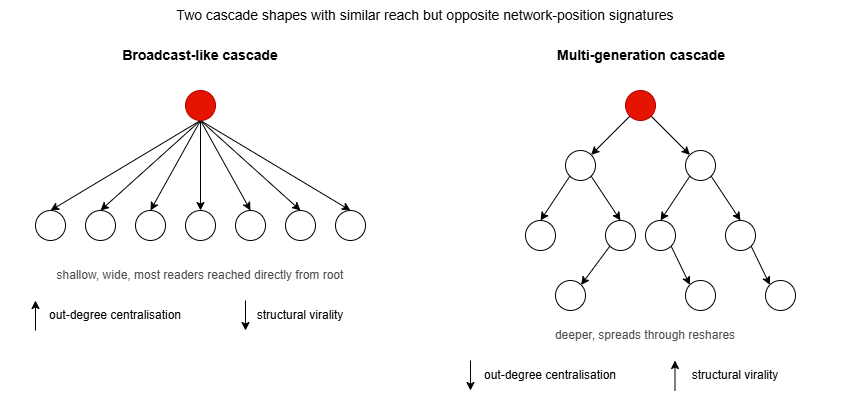
\includegraphics[width=0.92\textwidth]{figures/figure_3_1_cascade_shapes.png}
\caption{Two schematic cascade shapes with different network-position signatures.}
\label{fig:3-1}
\caption*{Note. The schematic contrasts a broadcast-like cascade with a multi-generation cascade. It is used to clarify the interpretation of depth, structural virality, and out-degree centralisation, not to report an empirical case.}
\end{figure}

At the content level, the primary outcome is \varname{log\_reach}, defined as:
\begin{equation}
\varname{log\_reach}
= \log(1 + \varname{cascade\_size}).
\end{equation}

Here, \varname{cascade\_size} measures the observed reach of an article–agent diffusion case. It represents the number of reader records reached through the reconstructed cascade generated by one article shared by one agent. The log transformation is used because diffusion reach is highly skewed: most article–agent cases generate limited reach, while a smaller number produce much larger cascades. Using log(1 + x) preserves zero and low-count observations while reducing the influence of extreme values. It measures how far a particular article–agent sharing case travelled.

The Level 1 supplementary outcomes describe the shape and engagement pattern of the same article–agent diffusion case. These include first- and second-layer width, diffusion depth, resharing behaviour, reading duration, structural virality, and the Wiener index. These variables are not treated as ordinary predictors of reach in the content-level analysis. Instead, they represent alternative diffusion outcomes, such as whether a cascade is broad, deep, reshared, or structurally more dispersed. Centrality-class outcomes are excluded from Level 1 because a centrality measure does not have a clean interpretation as a content-level outcome for a single article–agent case.

At the agent-characteristic level, the primary outcome is agent-level mean log reach, defined as:
\begin{equation}
\varname{log\_agent\_cascade\_size\_mean}
= \log(1 + \varname{cascade\_size\_mean}).
\end{equation}

Here, \varname{cascade\_size\_mean} is the agent’s average cascade size across the article–agent cases associated with that agent. This outcome summarises an agent’s typical reach performance, not the reach of any individual share. The log transformation again reduces skewness and supports comparison across agents with different average diffusion scales.

The Level 2 supplementary outcomes capture different aspects of agent-level diffusion behaviour. These include average depth, average second-layer width, mean reshare behaviour, mean reading duration, structural virality, the Wiener index, centrality-related measures, repeat-exposure measures, and network-composition measures such as gender assortativity. At this level, reconstructed network-position measures such as centrality have a coherent interpretation because they are aggregated across an agent’s observed sharing activity.

At the content–agent matching level, the primary outcome is agent–topic mean log reach, defined as:
\begin{equation}
\varname{log\_agent\_topic\_cascade\_size\_mean}
= \log(1 + \varname{cascade\_size\_mean}).
\end{equation}

In this case, \varname{cascade\_size\_mean} is calculated within each agent–topic pair. The outcome measures the average reach of articles in a particular topic when shared by a particular agent. This is the most direct outcome for the matching analysis because the central question is whether stronger fit between an agent’s professional context and a content topic is associated with stronger diffusion performance for that agent–topic combination.

The Level 3 supplementary outcomes use the same logic at the agent–topic level. They include agent–topic averages of depth, second-layer width, reshare behaviour, reading duration, structural virality, the Wiener index, and centrality-related measures where these are meaningful after aggregation. These outcomes allow the matching analysis to examine whether content–agent fit is associated not only with reach, but also with different diffusion shapes and engagement patterns.

The use of different outcome names across levels does not mean that the dissertation changes its core concept of diffusion effectiveness. Each outcome adapts the same reach-based idea to the relevant unit of analysis. Supplementary outcomes then show that diffusion effectiveness includes more than reach alone, while preserving the level-specific interpretation of each metric.

\section{Data Limitations}
\label{sec:3-6-data-limitations}

The limitations discussed here concern the scope and observability of the data themselves. They define what the WeiMai records can and cannot show. The processing steps used to construct variables from these records are described in Chapter 4, while the implications for interpretation, generalisability, and future research are discussed in Chapter 8.

First, the dataset is observational. The records are behavioural traces generated by a real WeiMai marketing operation, not data produced by a controlled experiment. Articles were not randomly assigned to agents. This means that the data record observed sharing, reading, and resharing behaviour, but do not contain an experimental assignment mechanism that would allow causal identification.

Second, the data come from a single firm in the interior-design and home-decoration industry. This provides a coherent empirical context for studying content–agent fit, but it also means that the raw data represent one organisational setting, one industry context, and one platform-mediated marketing system. The dataset does not include comparable firms from other sectors or parallel marketing campaigns from other platforms.

Third, the behavioural records capture platform-recorded activity only. They include fields such as reading time, dwell time, resharing indicators, reader layer, and parent-linkage information, but they do not observe readers’ motivations, prior topic interests, offline interactions, or perceptions of the agent who shared the article. Similarly, the data do not observe the full composition of each agent’s WeChat audience. These unobserved factors may matter for diffusion but are not available in the dataset.

Fourth, the final empirical datasets depend on linkage across behavioural records, article content files, and agent profile or identifier records. Records that cannot be linked consistently across these sources are excluded from the final analytical scope. This improves internal consistency but means that the analysis is based on cleaned and linkable subsets of the original platform records, not on every raw record in the database.

Fifth, diffusion analysis depends on the linkage information recorded by the platform. Reader-layer and parent-linkage fields make it possible to reconstruct observed propagation paths, but they only describe activity captured inside the platform records. Sharing, exposure, or interaction that occurred outside the recorded WeiMai environment cannot be recovered from the data.

Sixth, the article source material is unstructured. The raw article corpus consists of DOCX files containing titles, body text, and embedded images, but it does not contain pre-existing topic labels, title–content consistency scores, or standardised image-use variables. These features must be constructed before they can be analysed.

Seventh, the agent profile data are limited. Job titles and department information provide observable indicators of professional context, but they do not capture the full content of each agent's work, seniority, expertise, client base, or audience composition. Agent gender is not directly recorded in the profile data, which is inferred from agent names and coded as a categorical attribute.

Eighth, the agent–topic data are sparse. Although the matching dataset contains 1,142 agent–topic pairs, many pairs are supported by few underlying article–agent cases. The median pair is supported by two cases; 379 pairs are supported by a single case; 126 pairs have at least ten cases; and 46 pairs have at least thirty cases. Average outcomes for sparsely populated pairs are less stable than averages based on many cases.

Finally, some model-specific samples are smaller than the master dataset row counts because not every observation has complete information on every variable needed for every specification. For example, the content-level master dataset contains 6,557 article–agent cases, while the main content regression uses 6,556 complete cases.
